\clearpage
\section{Implementation}

\subsection{Data Collection}

We conducted a short \acrfull{eda} on a daily-interval dataset spanning 
from 2024-01-01 to 2025-03-28, which contains 2,820 records without missing values.
This process offers initial insights into basic descriptive statistics, volatility measures,
and technical indicators. Interested readers can refer to the Appendix~\ref{app:eda}.

\subsection{Feature Selection}

In Table~\ref{tab:feature_selection}, we exclude extra, highly correlated, or readily derived
indicators to maintain a simpler and more efficient feature set. This approach enhances model
performance by minimizing noise and reducing redundant information during training.

\begin{table}[H]
\centering
\caption{Feature Selection}
\label{tab:feature_selection}
\begin{tabular}{ccp{2cm}p{6cm}}
\hline
\textbf{Category} & \textbf{Feature to Keep} & \textbf{Feature to Remove} & \textbf{Reason} \\
\hline\hline
\textbf{Momentum}  & \acrshort{ema} & \acrshort{sma}, \acrshort{wma} & 
\acrshort{ema} updates faster than \acrshort{sma}/\acrshort{wma}, providing a more 
responsive measure of price changes.\\
\textbf{Trend}     & \acrshort{macd} & \acrshort{macd} Signal & 
\acrshort{macd} itself is a good summary of trend changes. The signal can be
derived from \acrshort{macd} if needed, minimizing overlapping information. \\
\textbf{Volatility} & \acrshort{bb} (Middle) & \acrshort{bb} (Lower / Upper) & Keeping the 
middle band captures the moving average component; the lower/upper bands are derivable from the
middle band plus standard deviation, so we omit them to streamline features.\\
\hline
\end{tabular}
\end{table}

Details about the indicators are provided in Table~\ref{tab:docind}. Also the dataset with all the features
selected are in Table~\ref{tab:dataset_structure}.

\subsection{Data Splitting Strategy}

To ensure robust model evaluation while preserving the temporal nature of stock data, the
dataset was split chronologically into training, validation, and test sets using a 
75\% / 15\% / 15\% ratio. This approach prevents look-ahead bias, as the model is always
trained on past data and evaluated on future data it has not seen.

The dataset spans from 2014-01-02 to 2025-03-28, comprising 2,820 daily observations of
WDAY stock prices and associated technical indicators. Summary details for each split are provided in Table~\ref{tab:data-split-summary}.

\begin{table}[H]
\centering
\caption{Dataset Split Summary}
\label{tab:data-split-summary}
\begin{tabular}{lcccc}
\hline
\textbf{Set} & \textbf{Start Date} & \textbf{End Date} & \textbf{Records} & \textbf{Ratio} \\
\hline\hline
\textbf{Training}     & 2014-01-02 & 2021-11-08 & 1,973 & 75\% \\
\textbf{Validation}   & 2021-11-09 & 2023-07-20 & 424   & 15\% \\
\textbf{Test}         & 2023-07-21 & 2025-03-28 & 423   & 15\% \\
\hline
\end{tabular}
\end{table}

\subsection{Data Normalization:}
All feature normalization is applied \emph{after} splitting the dataset into 
training, validation, and test sets. This design choice is crucial to prevent 
information from the validation or test sets from leaking into the training 
process, a phenomenon known as \emph{data leakage}.

For normalization, this study employs the \texttt{MinMaxScaler} from 
\texttt{scikit-learn}, which scales features to a fixed range of $[0, 1]$. The 
scaler is \emph{fit exclusively on the training set to capture the scale parameters 
(i.e., minimum and maximum values) from the training data only}. These same 
parameters are then used to transform the validation and test sets. This ensures 
that no future information (i.e., from unseen data) influences the training 
process, thereby \emph{preserving the integrity and generalization of the 
model's evaluation}.

\subsection{Model Architectures and Hyperparameter Tuning}

Two deep learning architectures were selected for evaluation in this study: 

\begin{description}
    \item[\acrshort{lstm}] A stacked LSTM architecture with two LSTM layers, each followed by dropout, and a final dense 
    layer for output prediction. This structure enhances the model's ability to capture complex temporal dependencies in 
    financial time series, improving over single-layer baselines. Commonly adopted in stock forecasting due to its balance 
    of performance and simplicity \parencite{parmar2018stock, phuoc2024StockPrediction}.
    \item[\acrshort{lstmbigru}] A hybrid model combines a \acrshort{bigru} layer with a stack of three
    \acrshort{lstm} layers and intermediate dropout regularization. This deeper architecture is
    designed to capture both forward and backward temporal patterns as well as longer-term 
    dependencies within sequential data. Such hybrid recurrent networks have shown superior
    forecasting accuracy in recent works
    \parencite{shaban2024SMPDL, chang2024StockPrediction, guo2024LSTMStock}, particularly 
    when applied to volatile and non-stationary stock market data.
\end{description}

Figure~\ref{fig:model-comparison} illustrates the architectures of both models used in this 
study: the simple LSTM baseline and the LSTM-BiGRU hybrid model.

\begin{figure}[H]
\centering
\caption{Comparison of model architectures used in this study}
\label{fig:model-comparison}

\begin{subfigure}[t]{0.45\textwidth}
\centering
\caption{LSTM architecture}
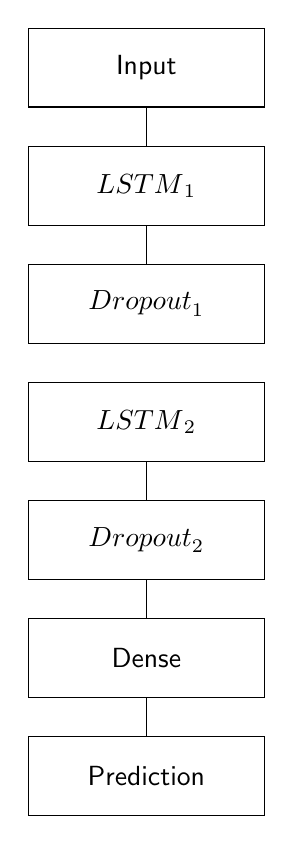
\begin{tikzpicture}[node distance=1.5cm, every node/.style={draw, minimum width=3cm, minimum height=1cm, font=\sffamily}, scale = 0.5]
\node (input) {Input};
\node (lstm1) [below of=input] {$\text{LSTM}_1$};
\node (drop1) [below of=lstm1] {$\text{Dropout}_1$};
\node (lstm2) [below of=drop1] {$\text{LSTM}_2$};
\node (drop2) [below of=lstm2] {$\text{Dropout}_2$};
\node (dense) [below of=drop2] {Dense};
\node (output) [below of=dense] {Prediction};
\draw (input) -- (lstm1);
\draw (lstm1) -- (drop1);
\draw (lstm2) -- (drop2);
\draw (drop2) -- (dense);
\draw (dense) -- (output);
\end{tikzpicture}
\end{subfigure}
%
\begin{subfigure}[t]{0.45\textwidth}
\centering
\caption{LSTM-BiGRU hybrid architecture}
\begin{tikzpicture}[node distance=1.5cm, every node/.style={draw, minimum width=3cm, minimum height=1cm, font=\sffamily}, scale = 0.5]
\node(input) {Input};
\node[below of=input] (bigru) {BiGRU};
\node[below of=bigru] (drop1) {$\text{Dropout}_1$};
\node[below of=drop1] (lstm1) {$\text{LSTM}_1$};
\node[below of=lstm1] (drop2) {$\text{Dropout}_2$};
\node[below of=drop2] (lstm2) {$\text{LSTM}_2$};
\node[below of=lstm2] (drop3) {$\text{Dropout}_3$};
\node[below of=drop3] (lstm3) {$\text{LSTM}_3$};
\node[below of=lstm3] (drop4) {$\text{Dropout}_4$};
\node[below of=drop4] (dense) {Dense};
\node[below of=dense] (output) {Prediction};
\draw[arrow] (input) -- (bigru);
\draw[arrow] (bigru) -- (drop1);
\draw[arrow] (drop1) -- (lstm1);
\draw[arrow] (lstm1) -- (drop2);
\draw[arrow] (drop2) -- (lstm2);
\draw[arrow] (lstm2) -- (drop3);
\draw[arrow] (drop3) -- (lstm3);
\draw[arrow] (lstm3) -- (drop4);
\draw[arrow] (drop4) -- (dense);
\draw[arrow] (dense) -- (output);
\end{tikzpicture}
\end{subfigure}
\end{figure}

Each model was trained using a supervised learning setup where the \emph{target variable is the next-day closing price}. 
Input features were normalized using \texttt{MinMaxScaler} prior to training. Hyperparameter optimization was performed 
using \texttt{Keras Tuner} with the \texttt{RandomSearch} strategy, enabling exploration of different model 
configurations such as layer sizes, dropout rates, and learning rates.

The hyperparameters explored in this study were informed by prior research, as
summarized in Table~\ref{tab:grid-search-hparams}.

\begin{table}[H]
\centering
\caption{Hyperparameter Configuration}
\label{tab:grid-search-hparams}
\begin{tabular}{lp{4.5cm}p{6cm}}
\hline
\textbf{Parameter} & \textbf{Values} & \textbf{Applies To} \\
\hline\hline
Model Type & \texttt{LSTM-BiGRU}, \texttt{LSTM} & Architecture \\
Hidden Units & \{16, 32, 64, 128\} & Number of recurrent units in each layer \\
Dense Units & \{16, 32\} & Number of units for Dense layers \\
Dropout Rate & \{0.01, 0.2, 0.3\} & Dropout applied after each layer \\
Learning Rate & \{0.0001, 0.001\} & Adam optimizer learning rate \\
Batch Size & \{64\} & Number of samples per gradient update \\
Scaler & \texttt{MinMaxScaler}& Input normalization method \\
Epochs & \{200\} & Max training epochs \\
Early Stopping & \begin{itemize}
    \item Patience = 10
    \item min\_delta = 1e-6
    \item monitor = \texttt{val\_loss}
    \item restore\_best\_weights = True
\end{itemize}  & Stops 
if no significant improvement for 10 epochs and reverts to best model, ignoring losses lower than $1e^{-6}$. \\
\hline
\end{tabular}
\end{table}

\subsection{Model Selection for LSTM and LSTM-BiGRU}

This section presents the final architectures and hyperparameters selected for both the 
\acrshort{lstm} and \acrshort{lstmbigru} models after completing hyperparameter tuning 
and model evaluation. While both models performed well, the \acrshort{lstmbigru} model 
achieved superior prediction accuracy on the test dataset. A full breakdown of the layer-wise 
parameters is provided in Appendix~\ref{app:modelshape}.

\subsubsection{Selected LSTM Model Configuration}

\begin{itemize}
  \item \textbf{Sequence Length}: 30
  \item \textbf{Hidden Units}:
    \begin{itemize}
      \item LSTM\textsubscript{1}: 128
      \item LSTM\textsubscript{2}: 32
    \end{itemize}
  \item \textbf{Dropout Rates}: 0.01 after each LSTM layer
  \item \textbf{Dense Layer}: 32 units
  \item \textbf{Learning Rate}: 0.001
  \item \textbf{Total Parameters}: 292,421
  \item \textbf{Trainable Parameters}: 97,473
\end{itemize}

\subsubsection{Selected LSTM-BiGRU Model Configuration}

\begin{itemize}
  \item \textbf{Sequence Length}: 30
  \item \textbf{Hidden Units}:
    \begin{itemize}
      \item BiGRU: 64
      \item LSTM\textsubscript{1}: 64
      \item LSTM\textsubscript{2}: 32
      \item LSTM\textsubscript{3}: 16
    \end{itemize}
  \item \textbf{Dropout Rates}: 0.01, 0.3, 0.2, 0.01 after each layer respectively
  \item \textbf{Dense Layer}: 16 units
  \item \textbf{Learning Rate}: 0.001
  \item \textbf{Total Parameters}: 293,669
  \item \textbf{Trainable Parameters}: 97,889
\end{itemize}

\subsubsection{Training Performance Comparison}

\begin{table}[H]
\centering
\caption{Architectural Comparison of Final Models}
\label{tab:model-comparison}
\begin{tabular}{lcc}
\hline
\textbf{Metric} & \textbf{LSTM} & \textbf{LSTM-BiGRU} \\
\hline\hline
Architecture Depth        & 2 LSTM layers           & BiGRU + 3 LSTM layers \\
Trainable Parameters      & 97,473                  & 97,889 \\
Total Parameters          & 292,421                 & 293,669 \\
Dropout Configuration     & Uniform (0.01)          & Layer-specific (0.01–0.3) \\
Feature Extraction        & Moderate                & Bidirectional \& hierarchical \\
\hline
\end{tabular}
\end{table}


\begin{figure}[H]
\centering
\caption{LSTM Training Metrics: (a) Loss (MSE), (b) Mean Squared Error, (c) Mean Absolute Error, (d) $R^2$ Score.}
\label{fig:lstm-training-performance}
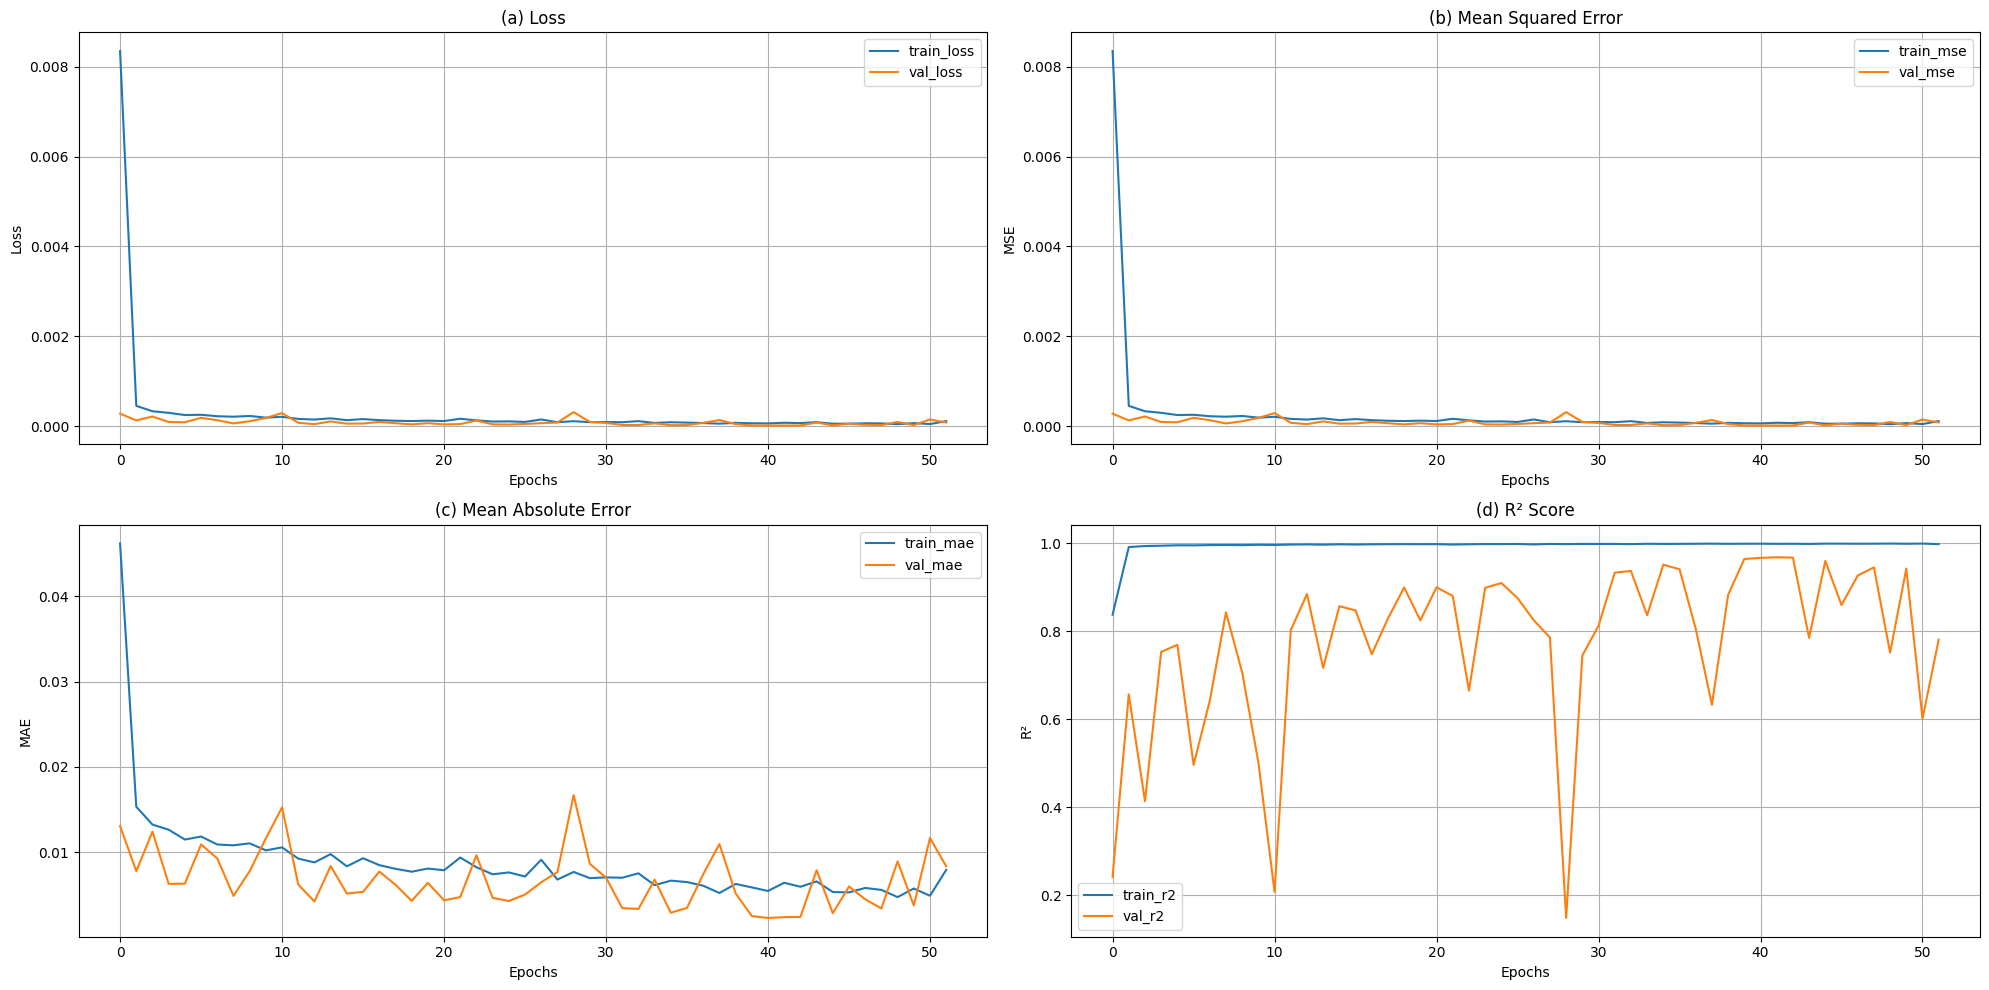
\includegraphics[width=\textwidth]{img/sections/main/best_lstm_training.png}
\end{figure}

\begin{figure}[H]
\centering
\caption{LSTM-BiGRU Training Metrics: (a) Loss (MSE), (b) Mean Squared Error, (c) Mean Absolute Error, (d) $R^2$ Score.}
\label{fig:bigru-training-performance}
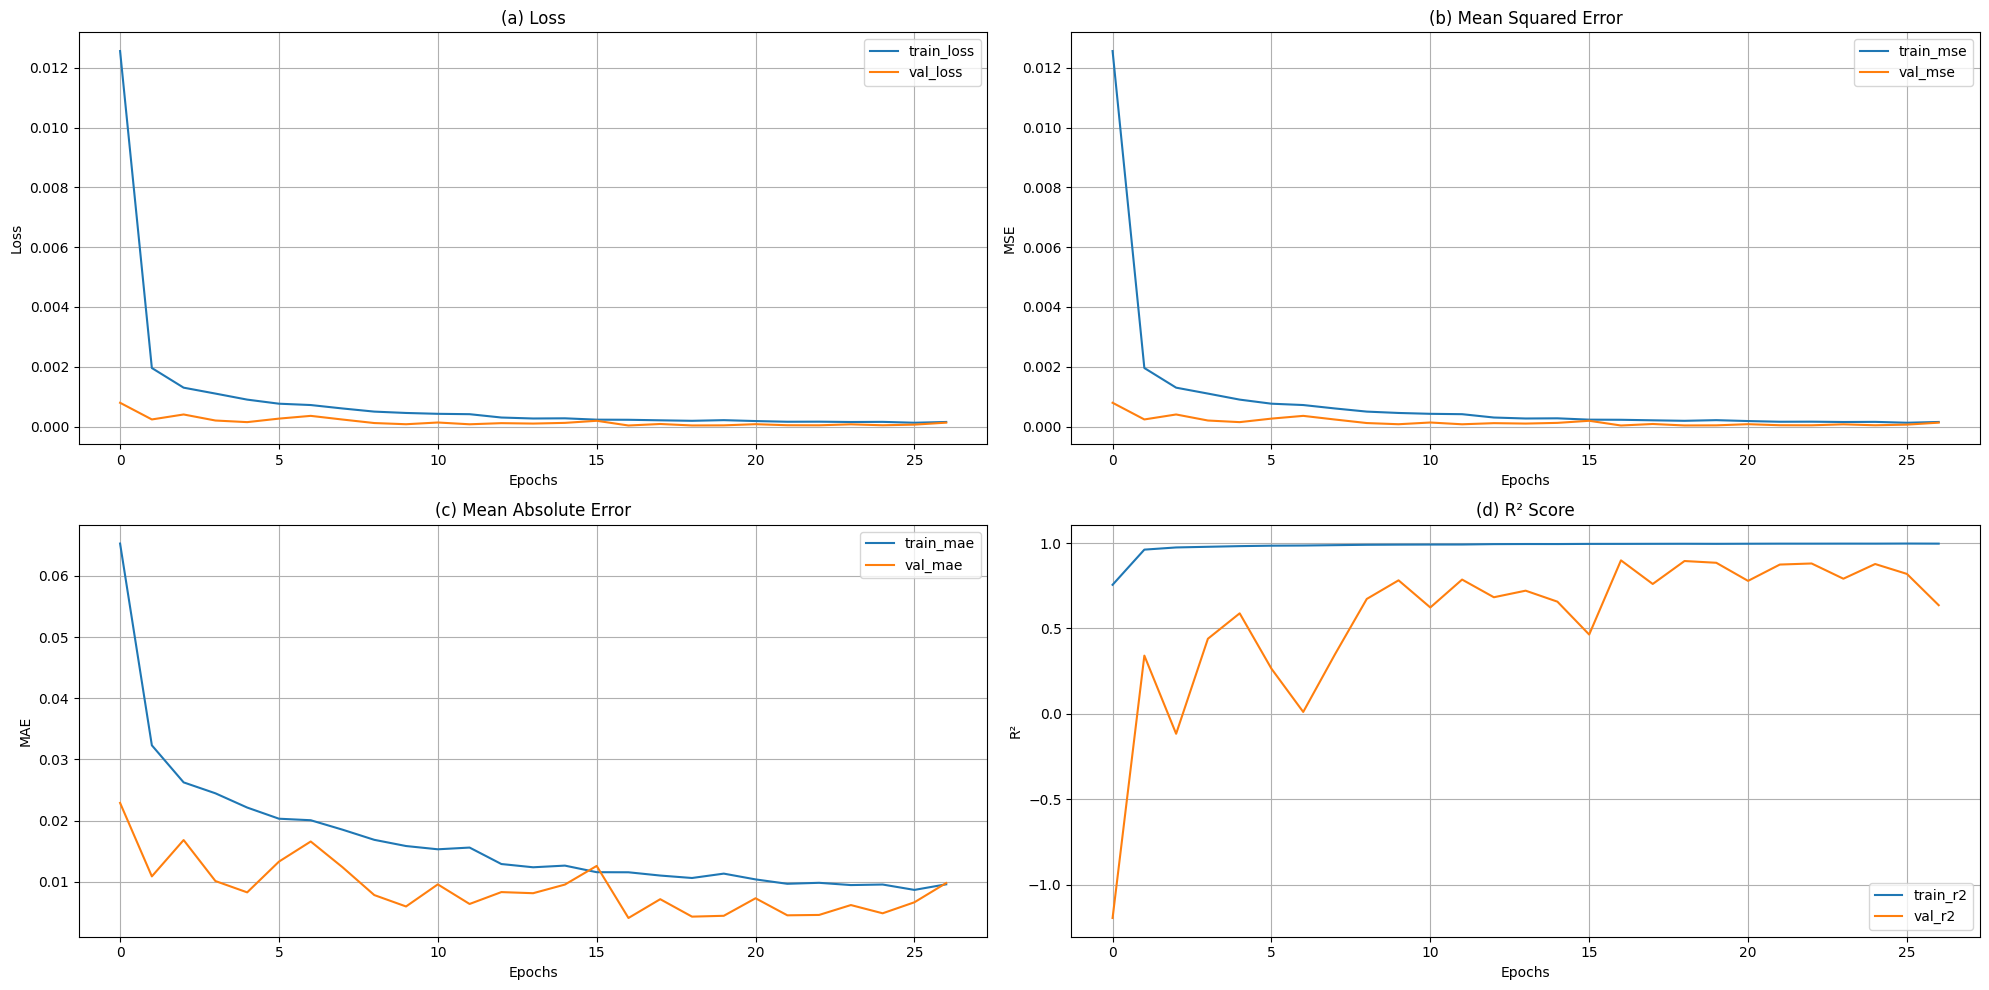
\includegraphics[width=\textwidth]{img/sections/main/best_lstmbigru_training.png}
\end{figure}

Both models demonstrated strong performance in predicting next-day stock prices, as evidenced by their low loss values.

\begin{description}
    \item[Training Convergence \& Generalization] 
        \leavevmode\\[1em]
        \textbf{LSTM:} The \acrshort{lstm} model (Figure~\ref{fig:lstm-training-performance}) achieved
            steady convergence with 
            validation metrics closely tracking training metrics. The \acrshort{r2} score stabilizes around 0.85 - 0.95, 
            indicating strong predictive power and minimal overfitting. \acrshort{mse} and \acrshort{mae} also 
            consistently decreased, demonstrating stable learning behavior.
        \leavevmode\\[1em]
        \textbf{LSTM-BiGRU:} The \acrshort{lstmbigru} model (Figure~\ref{fig:bigru-training-performance}), while 
        trained for fewer epochs, exhibited 
        faster convergence and even higher validation performance, with 
        an \acrshort{r2}, improves steadily, reaching above 0.9 in 
        later epochsvindicating the 
        model is explaining a high proportion of variance in the target 
        variable on unseen data.
    \item[Architecture Efficiency] 
        \leavevmode\\[1em]
        \textbf{LSTM \& LSTM-BiGRU:} Despite the increased architectural complexity, the \acrshort{lstmbigru} model
        maintained a similar number of trainable parameters as the \acrshort{lstm} model (97,889 vs. 97,473), 
        indicating efficient use of network depth and gating mechanisms. The \acrshort{bigru} component enables the 
        model to consider both forward and backward dependencies, which is especially useful in 
        financial time-series where future trends often mirror past volatility patterns.
    \item[Dropout Rates \& Dataset Size] 
        \leavevmode\\[1em]
        \textbf{LSTM \& LSTM-BiGRU:} 
        An interesting observation lies in the chosen dropout rates. Both models 
        employed a relatively low dropout rate of 0.01, while the \acrshort{lstmbigru} model introduced variation 
        across layers, ranging from 0.01 to 0.3. This minimal level of regularization can be justified by the limited 
        size of the training dataset, which spans a 10-year period of daily stock prices. In smaller datasets, 
        overly aggressive dropout may cause underfitting, as it restricts the model's learning capacity. Conversely, 
        lower dropout helps preserve essential temporal features. Moreover, the use of optimization strategies such 
        as the Adam optimizer and early stopping (with patience and weight restoration) further mitigates the 
        risk of overfitting, providing additional robustness to the training process. 
\end{description}

\paragraph{Summary of Results} The experimental results clearly indicate that the \emph{\acrshort{lstmbigru} model 
outperforms the standalone \acrshort{lstm} across all key evaluation metrics}, including \acrshort{mse}, 
\acrshort{mae}, and \acrshort{r2}. While the \acrshort{lstm} model demonstrated stable convergence and strong
predictive capabilities, the hybrid \acrshort{lstmbigru} architecture achieved faster convergence.
